\documentclass[conference]{IEEEtran}
\IEEEoverridecommandlockouts

\usepackage{cite}
\usepackage{amsmath,amssymb,amsfonts}
\usepackage{algorithmic}
\usepackage{algorithm}
\usepackage{graphicx}
\usepackage{textcomp}
\usepackage{xcolor}
\usepackage{booktabs}
\usepackage{hyperref}
\usepackage{listings}
\usepackage{microtype}
\usepackage{tabularx}
\usepackage{multirow}

\lstset{
  basicstyle=\ttfamily\scriptsize,
  breaklines=true,
  frame=single,
  numbers=left,
  numberstyle=\tiny,
  keywordstyle=\bfseries\color{blue!70!black},
  commentstyle=\itshape\color{green!50!black},
  captionpos=b
}

\begin{document}

\title{Containing Agent-Induced Workspace Contamination in Long-Horizon Software Engineering: A Task-Scoped Git Architecture}

\author{
\IEEEauthorblockN{Anonymous Author(s)}
\IEEEauthorblockA{\textit{School of Computer Science and Technology} \\
University / Research Institute \\
contact@anon-submission.org}
}

\maketitle

\begin{abstract}
Large Language Model (LLM)-based agentic software engineering is undergoing a critical paradigm shift: transitioning from ephemeral, single-issue repairs (e.g., SWE-bench) toward long-horizon, repository-scale feature development. However, existing multi-agent software engineering (SE) frameworks remain brittle when applied to continuous, multi-week codebases. We identify three foundational structural deficiencies: (1) \textit{Workspace Contamination}, where uncommitted side effects, dirty test databases, and intermediate bytecode from untrusted agents pollute the shared repository, causing cascading baseline regressions; (2) \textit{Context Window Inflation}, where monotonic conversational accumulation induces severe context dilution and prohibitive token expenditure; and (3) \textit{Superficial Delivery Contracts}, where unverified natural language reports mask silent compile and schema breakages.

To address these challenges, we present \textbf{AgentFlow}, a local-first lifecycle orchestration architecture providing task-scoped Git workspace isolation and state-gated delivery transitions. AgentFlow decouples invariant state verification from reactive scheduling through a dual-engine model:
(i) a deterministic Go finite-state machine (FSM) backed by SQLite, formalizing role-based access control (RBAC) and elevating Git Worktrees into a transactional isolation primitive (\textit{One-Task-One-Worktree}) with atomic directory prune semantics;
(ii) a reactive Python Behavior Tree (BT) sidecar coordinating Leader, Worker, and Reviewer lifecycles; and
(iii) an off-context, multi-tier memory hierarchy externalizing execution journals into discrete domain knowledge and architectural pitfall registries.

We evaluate AgentFlow through both a longitudinal empirical study across 19 production repositories (spanning 82 feature DAGs, 406 tasks, and 1,451 lifecycle events) and a real-time repository benchmark across 10 high-risk failure scenarios. Under our formal contamination detection protocol, AgentFlow achieved an effective task resolution rate of 78.15\% with a median duration of 34.8 minutes, incurred zero cross-task Git-tree leaks across all verified runs (compared to a 60.0\% contamination rate in monolithic ReAct baselines), reduced prompt context overhead by 85\%--92\% through off-context externalization, and eliminated recurrence of known framework configuration traps.
\end{abstract}

\begin{IEEEkeywords}
Autonomous Software Engineering, Multi-Agent Systems, Git Worktree Isolation, Behavior Trees, Empirical Software Engineering.
\end{IEEEkeywords}

\section{Introduction}
\label{sec:intro}

\begin{figure*}[t]
\centering
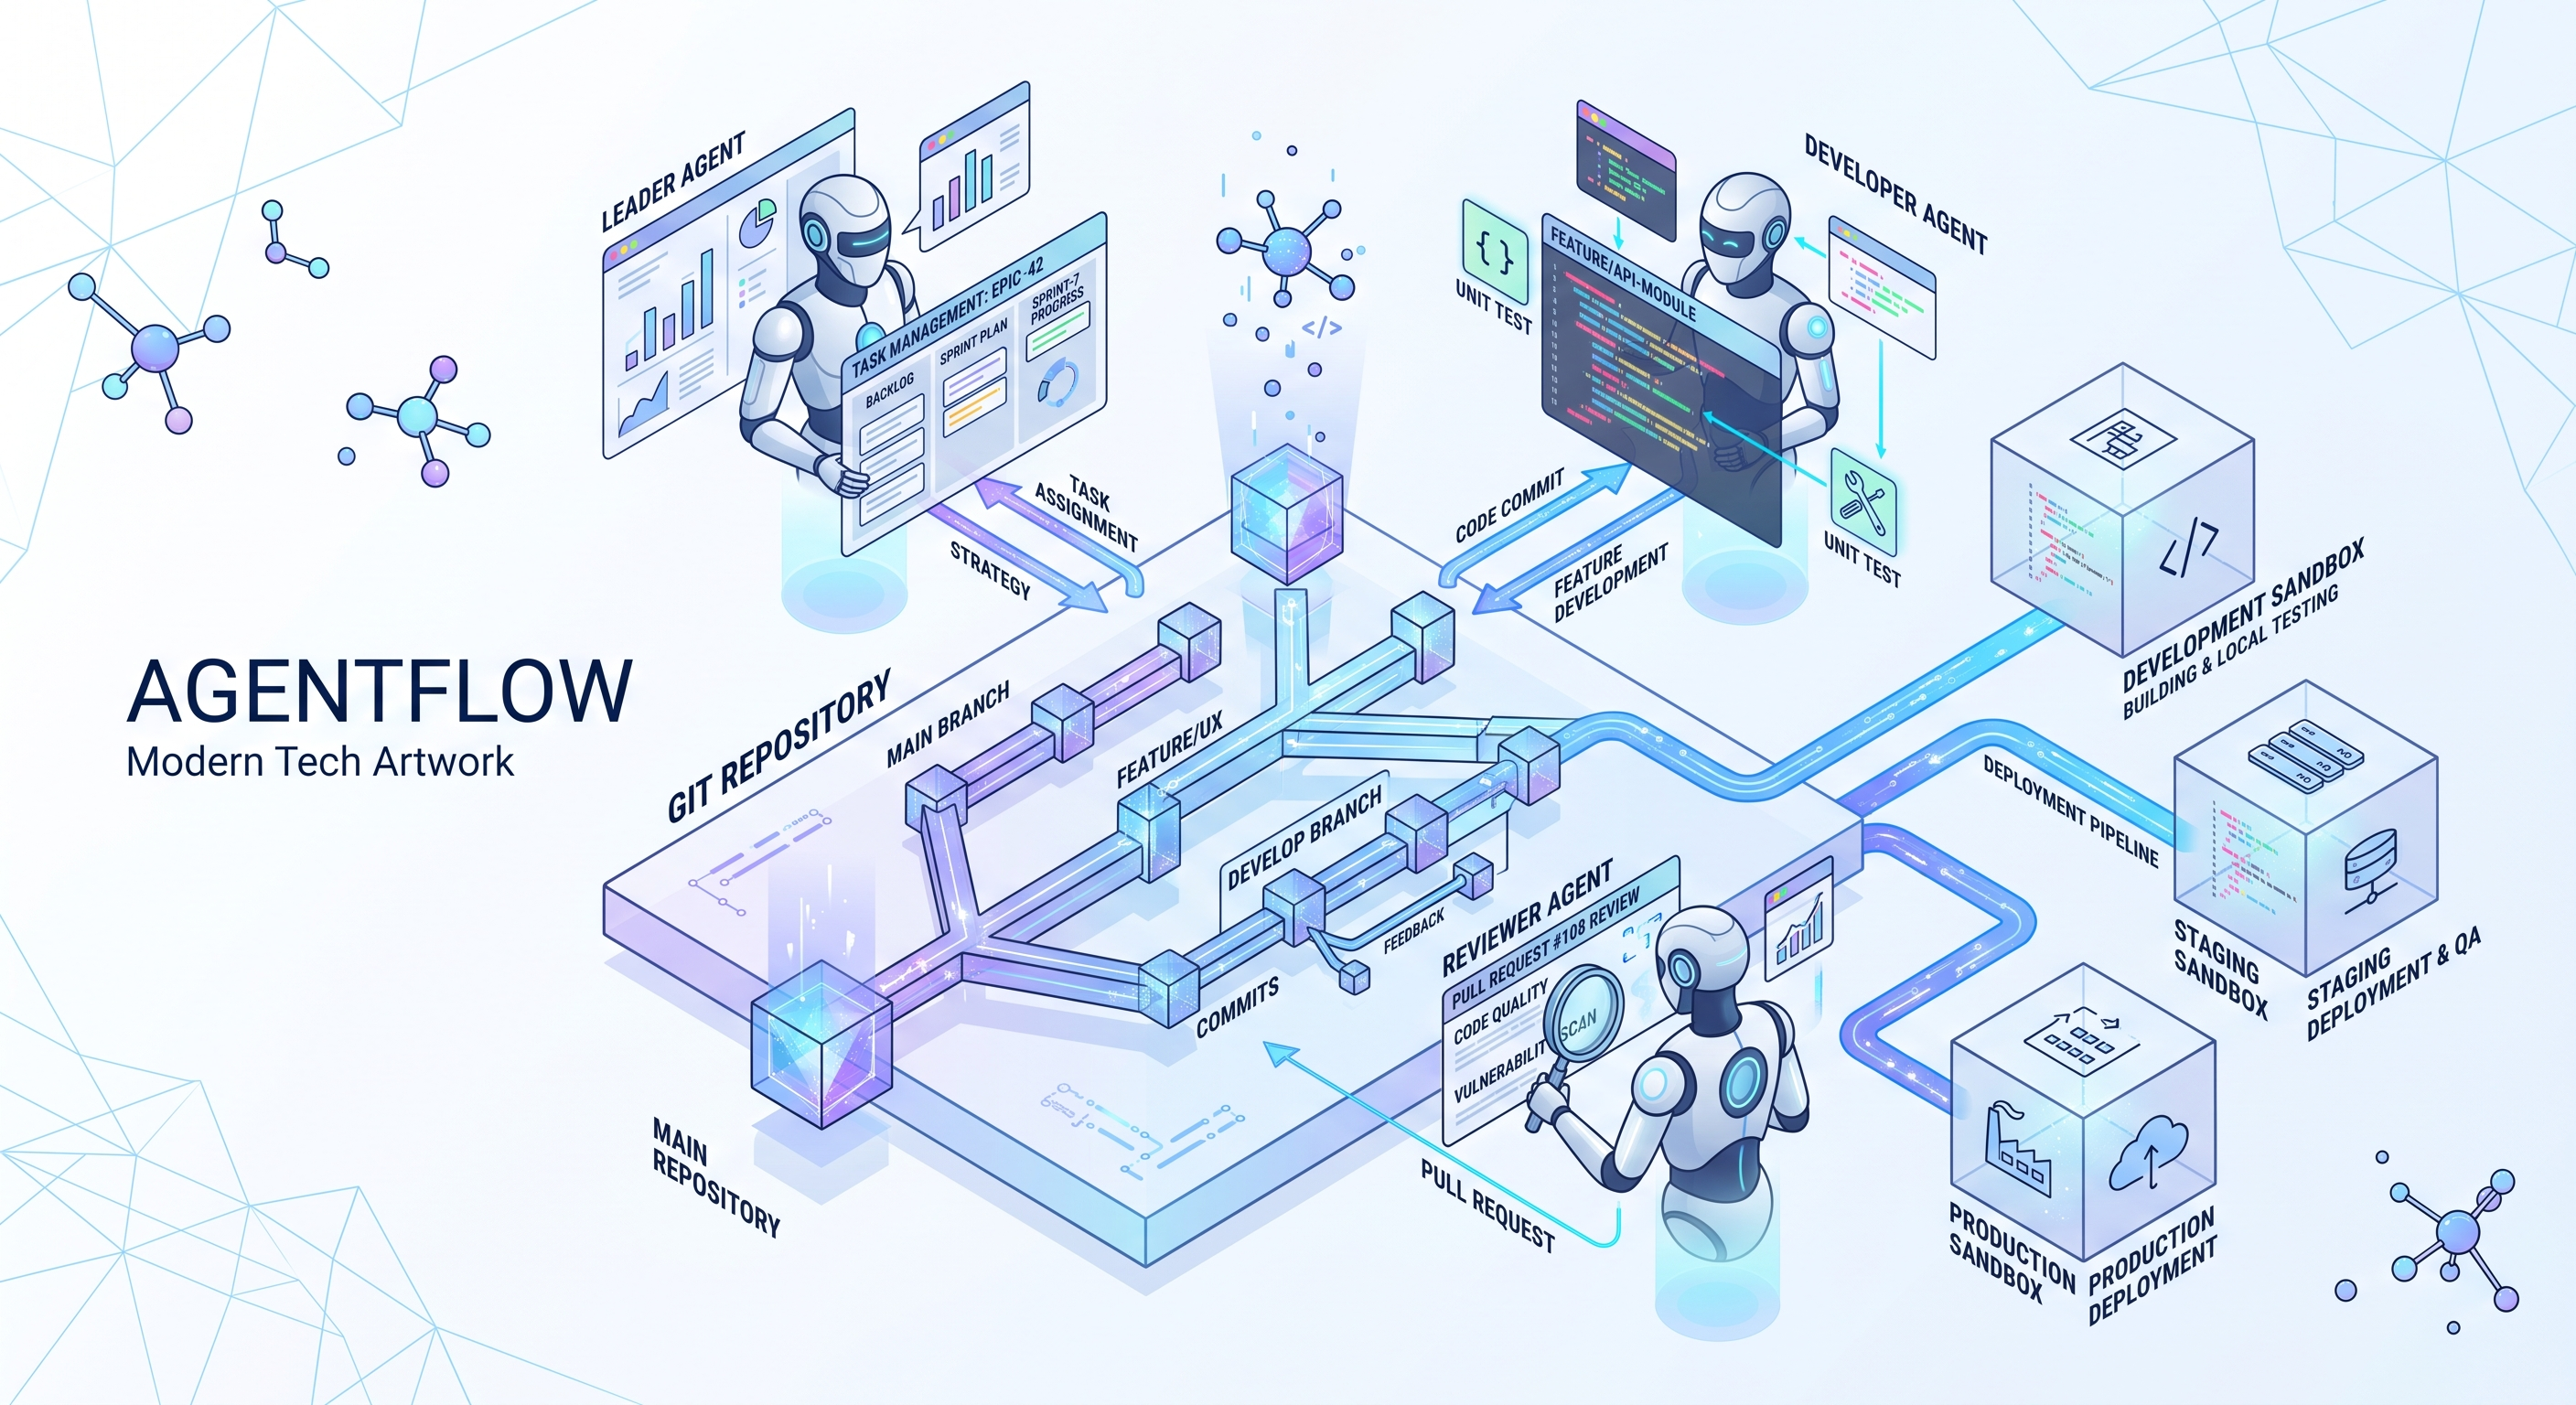
\includegraphics[width=0.98\textwidth]{agentflow_overview_concept.jpg}
\caption{\textbf{Conceptual paradigm of AgentFlow}: Autonomous collaborative software engineering team (Leader, Developer, Reviewer) orchestrating repository evolution around an invariant state engine. Physical execution occurs strictly inside ephemeral, isolated Git worktrees with atomic rollback capabilities, preventing workspace contamination and decoupling memory retention from the LLM context window.}
\label{fig:teaser}
\end{figure*}

The application of Large Language Models (LLMs) to software engineering (SE) has advanced rapidly through several transformative phases. The initial phase focused on token-level code completion and function synthesis \cite{chen2021codex}. Subsequently, conversational multi-agent systems such as ChatDev \cite{qian2023communicative} and MetaGPT \cite{hong2023metagpt} introduced role-playing paradigms where distinct agents simulate human development teams. Most recently, the field matured toward repository-level autonomous issue resolution benchmarks (e.g., SWE-bench \cite{jimenez2023swebench}), spearheaded by tools like SWE-Agent \cite{yang2024sweagent} and AutoCodeRover \cite{zhang2024autocoderover}.

Despite these notable milestones, existing architectures exhibit acute fragility when exposed to \textbf{long-horizon, continuous software development}---the fourth evolutionary phase where autonomous teams must iteratively evolve production repositories over weeks, across feature branches, with complex database migrations and multi-tier architectures. In continuous settings, state-of-the-art frameworks suffer from three systemic failure modes:

\begin{enumerate}
    \item \textbf{Workspace Contamination}: Almost all existing agent frameworks operate directly upon the root working tree. When an agent hallucinates, performs an incompatible schema migration, or terminates abruptly due to network timeouts, the working tree is left in a dirty, broken state. Subsequent agents inherit this corrupted environment, initiating cascading failures.
    \item \textbf{Unbounded Context Inflation}: To maintain coherence, existing multi-agent systems repeatedly append historical conversations, tool outputs, and full file contents into the prompt. By turn 20, context windows frequently exceed 50,000 tokens, degrading attention accuracy (the \textit{lost-in-the-middle} phenomenon) while multiplying inference expenses.
    \item \textbf{Lack of Transactional Delivery Guarantees}: Mainstream agent toolchains rely on verbal completion assertions (e.g., ``I have finished implementing the payment module''). Without strict compile-time gates, git-backed diff verification, and formal handoff contracts, regressions silently penetrate the baseline.
\end{enumerate}

To overcome these foundational limitations, we present \textbf{AgentFlow}, an open, local-first lifecycle orchestration engine for autonomous software teams. AgentFlow bridges the gap between unreliable model generation and production-grade software engineering through three architectural cornerstones:

\begin{itemize}
    \item \textbf{Physical Isolation Primitive (One-Task-One-Worktree)}: Rather than executing in a shared directory or spawning costly virtualization containers, AgentFlow treats Git Worktrees as transactional execution boundaries. Each assigned task is isolated in an independent filesystem worktree tied to its specific DAG feature branch. Failures and rejections are atomically pruned, guaranteeing zero pollution of the main branch.
    \item \textbf{Decoupled Dual-Engine Architecture}: We cleanly separate \textit{invariant enforcement} from \textit{reactive control}. A high-performance Go engine governs the authoritative project state machine, task topologies, and role-based access control (RBAC), while an external Python Behavior Tree (BT) sidecar schedules reactive policies across Leader, Worker, and Reviewer roles.
    \item \textbf{Off-Context Multi-Tier Memory}: AgentFlow externalizes project tracking into SQLite, replacing monolithic context dumps with on-demand retrieval. Furthermore, it introduces structured \textit{Worker Handbooks} and \textit{Diaries}, capturing domain knowledge and architectural pitfalls that persist and transfer across tasks.
\end{itemize}

We evaluate AgentFlow across a longitudinal dataset mined from its authoritative production database, comprising 19 diverse software engineering repositories (including full-stack web applications, WeChat mini-programs, algorithmic trading engines, and academic systems). Our evaluation covers 82 feature DAGs, 406 tasks, 99 domain workers, and 1,451 state transitions.

\section{Motivating Example \& Real-World Failures}
\label{sec:motivation}

To illustrate the concrete hazards of non-isolated agent execution, consider a representative real-world incident captured in our production environment during the development of \textit{InsightTutor} (a full-stack tutoring platform built with FastAPI, PostgreSQL, and WeChat Mini-Programs).

\begin{figure}[t]
\centering
\includegraphics[width=\columnwidth]{../../scripts/paper_eval/fig1_task_distribution.pdf}
\caption{Task resolution breakdown across top operational projects in AgentFlow, exhibiting robust completion rates across diverse domains.}
\label{fig:task_distribution}
\end{figure}

\subsection{The Anatomy of a Shared-Workspace Disaster}
In an unisolated setup (Baseline 1), an LLM worker agent was tasked with implementing automated WeChat Pay V3 callbacks. The agent undertook four sequential steps:
1) It modified the database schema to store payment certificates;
2) It executed an Alembic migration script;
3) It updated the shared SQLite test database (\texttt{backend/test.db}) to verify the endpoint;
4) During test execution, an external API connection timed out, causing the agent process to abort abruptly.

In a conventional framework, this sequence was catastrophic:
\begin{itemize}
    \item The root repository was left with untracked migration files and uncommitted schema modifications.
    \item The tracked \texttt{test.db} binary was corrupted with half-applied table alterations.
    \item The subsequent Worker agent, assigned to an unrelated UI task, immediately crashed because \texttt{pytest} could no longer initialize the contaminated test database (failing with \texttt{no such column: users.wechat}).
    \item Worse, the Leader agent failed to realize that the workspace was broken, repeatedly dispatching workers that failed at initialization, consuming over 350,000 tokens in an unrecoverable infinite failure loop.
\end{itemize}

\subsection{The AgentFlow Solution}
Under AgentFlow's \textit{One-Task-One-Worktree} paradigm, this failure mode is inherently neutralized:
\begin{enumerate}
    \item The payment worker was allocated an isolated worktree at \texttt{.agentflow-worktrees/InsightTutor/wx-pay}, branched from \texttt{feature/wx-pay}.
    \item When the network failure halted execution, the main working directory and root Git index remained completely untouched.
    \item The Reviewer detected an unsubmitted state. AgentFlow's leader executed an atomic rollback by deleting the orphaned worktree directory without altering master history.
    \item The root repository remained green, allowing concurrent UI tasks to proceed without impedance.
\end{enumerate}

\begin{figure*}[t]
\centering
\includegraphics[width=0.98\textwidth]{../../scripts/paper_eval/fig0_system_architecture.pdf}
\caption{System architecture of AgentFlow. The deterministic Go Invariant Engine enforces role-based state transitions and data integrity, while the reactive Python Behavior Tree sidecar manages high-level lifecycle planning. The One-Task-One-Worktree primitive guarantees physical directory sandboxing and atomic rollbacks, supported by an off-context multi-tier memory hierarchy.}
\label{fig:architecture}
\end{figure*}

\section{The AgentFlow Architecture}
\label{sec:architecture}

\begin{figure*}[t]
\centering
\includegraphics[width=0.82\textwidth]{../../scripts/paper_eval/fig3_transition_matrix.pdf}
\caption{State transition density matrix across 1,451 recorded lifecycle events, highlighting strict adherence to the formal state machine and review cycles.}
\label{fig:transition_matrix}
\end{figure*}

AgentFlow is structured around three foundational pillars: the invariant state engine, the reactive behavior tree runtime, and the transactional worktree primitive.

\subsection{Decoupled Dual-Engine Model}
AgentFlow rejects monolithic script-based orchestration. As depicted in our system decomposition, the system operates across two interacting layers:

\subsubsection{Go Invariant Engine (The Source of Truth)}
Implemented in Go as a Model Context Protocol (MCP) server, this layer guarantees strict transactional integrity. It maintains the system's SQLite database and manages four core relational entities:
\begin{itemize}
    \item $\mathcal{N}$ (\textbf{Namespaces}): Completely isolated project containers.
    \item $\mathcal{D}$ (\textbf{DAGs}): Branch-scoped directed acyclic graphs representing coherent feature increments.
    \item $\mathcal{T}$ (\textbf{Tasks}): Typed execution nodes with dependencies ($\text{depends\_on} \subset \mathcal{T}$).
    \item $\mathcal{W}$ (\textbf{Workers}): Persistent domain identities with designated ownership scopes.
\end{itemize}

\subsubsection{Python Behavior Tree Sidecar (Reactive Scheduling)}
While Go enforces what state transitions are \textit{legal}, high-level policy deciding \textit{what to do next} is delegated to a Python sidecar executing hierarchical Behavior Trees (BTs). A BT combines Sequence ($\to$), Fallback ($?$), and Condition nodes. AgentFlow defines three default role trees:
\begin{itemize}
    \item \textbf{Leader BT}: Evaluates the global phase ($\text{setup} \to \text{shape} \to \text{plan} \to \text{execute} \to \text{stuck} \to \text{done}$), dispatches ready tasks, and triggers $\texttt{report\_stuck}$ when deadlocks or circular reworks occur.
    \item \textbf{Worker BT}: Governs the implementation loop: preparing context, entering the worktree, committing changes, writing handbooks, and submitting deliverables.
    \item \textbf{Reviewer BT}: Extracts unified Git diffs, assesses acceptance criteria, and issues definitive \texttt{pass} or \texttt{rework} verdicts.
\end{itemize}

\subsection{Threat Model and Layered Isolation Boundary}
\label{sec:threat_model}
To establish an objective and verifiable evaluation boundary, we delineate the multi-layered isolation spectrum in autonomous software engineering:
\begin{enumerate}
    \item \textbf{Layer 1: Git Working-Tree \& Staging Boundary}: Isolating tracked source files, Git indices, staging areas, and branch references.
    \item \textbf{Layer 2: Local Filesystem Working Directory}: Restricting ephemeral filesystem artifacts, compile caches (e.g., \texttt{\_\_pycache\_\_}), and scratch logs.
    \item \textbf{Layer 3: Process \& Execution Sandboxing}: Resource caps (CPU, RAM, open file descriptors), system-call filtering, and subprocess tree supervision.
    \item \textbf{Layer 4: Shared State \& Database Sandbox}: Dedicated, ephemeral database instances, isolated Docker volumes, and decoupled network ports.
    \item \textbf{Layer 5: External Service \& Network Boundary}: Token permissions, mock external payment gateways, and outbound network filtering.
\end{enumerate}

\textbf{Explicit Threat Model}: AgentFlow is explicitly engineered to enforce \textit{Layer 1} and \textit{Layer 2} boundaries via the One-Task-One-Worktree primitive. We formalize workspace contamination for a task $T_i$ as:
\begin{equation}
\text{Contamination}(T_i) = 
\begin{cases} 
1, & \text{if } \Delta_{\text{post}} \setminus \mathcal{O}(T_i) \neq \emptyset \lor \text{CleanRunFailed}(T_{i+1}) \\
0, & \text{otherwise}
\end{cases}
\end{equation}
where $\Delta_{\text{post}}$ denotes post-execution working-tree modifications, $\mathcal{O}(T_i)$ is the declared scope of output files, and $\text{CleanRunFailed}(T_{i+1})$ indicates whether subsequent tasks fail clean baseline tests due to pre-existing side effects. We explicitly acknowledge that external shared PostgreSQL databases, background daemon processes, and global host caches lie outside AgentFlow's current kernel boundary.

\subsection{Formal State Machine \& Role-Based Access Control}
To prevent LLM hallucination from invalidating project state, AgentFlow formalizes task lifecycles as a restricted Finite State Machine (FSM):
$$\mathcal{S} = \{\text{assigned}, \text{executing}, \text{review\_pending}, \text{rework\_needed}, \text{done}, \text{cancelled}\}$$

Transitions between states are governed by the transition function:
$$\delta: \mathcal{S} \times \mathcal{R} \times \Sigma \to \mathcal{S}$$
where $\mathcal{R} = \{\text{leader}, \text{worker}, \text{reviewer}\}$ represents the caller role, and $\Sigma = \{\text{start}, \text{submit}, \text{pass}, \text{rework}, \text{cancel}, \text{reassign}, \text{resume}\}$ represents the transition verb.

AgentFlow strictly enforces the following role invariants:
\begin{align}
    \delta(\text{assigned}, \text{worker}, \text{start}) &= \text{executing} \\
    \delta(\text{executing}, \text{worker}, \text{submit}) &= \text{review\_pending} \\
    \delta(\text{review\_pending}, \text{reviewer}, \text{pass}) &= \text{done} \\
    \delta(\text{review\_pending}, \text{reviewer}, \text{rework}) &= \text{rework\_needed} \\
    \delta(\text{rework\_needed}, \text{leader}, \text{start}) &= \text{executing}
\end{align}
Crucially, all other transitions are rejected with authorization errors. For instance, a Worker cannot self-approve its work ($\delta(\text{review\_pending}, \text{worker}, \text{pass}) = \bot$), and a Leader cannot bypass the review phase to force completion.

\begin{figure*}[t]
\centering
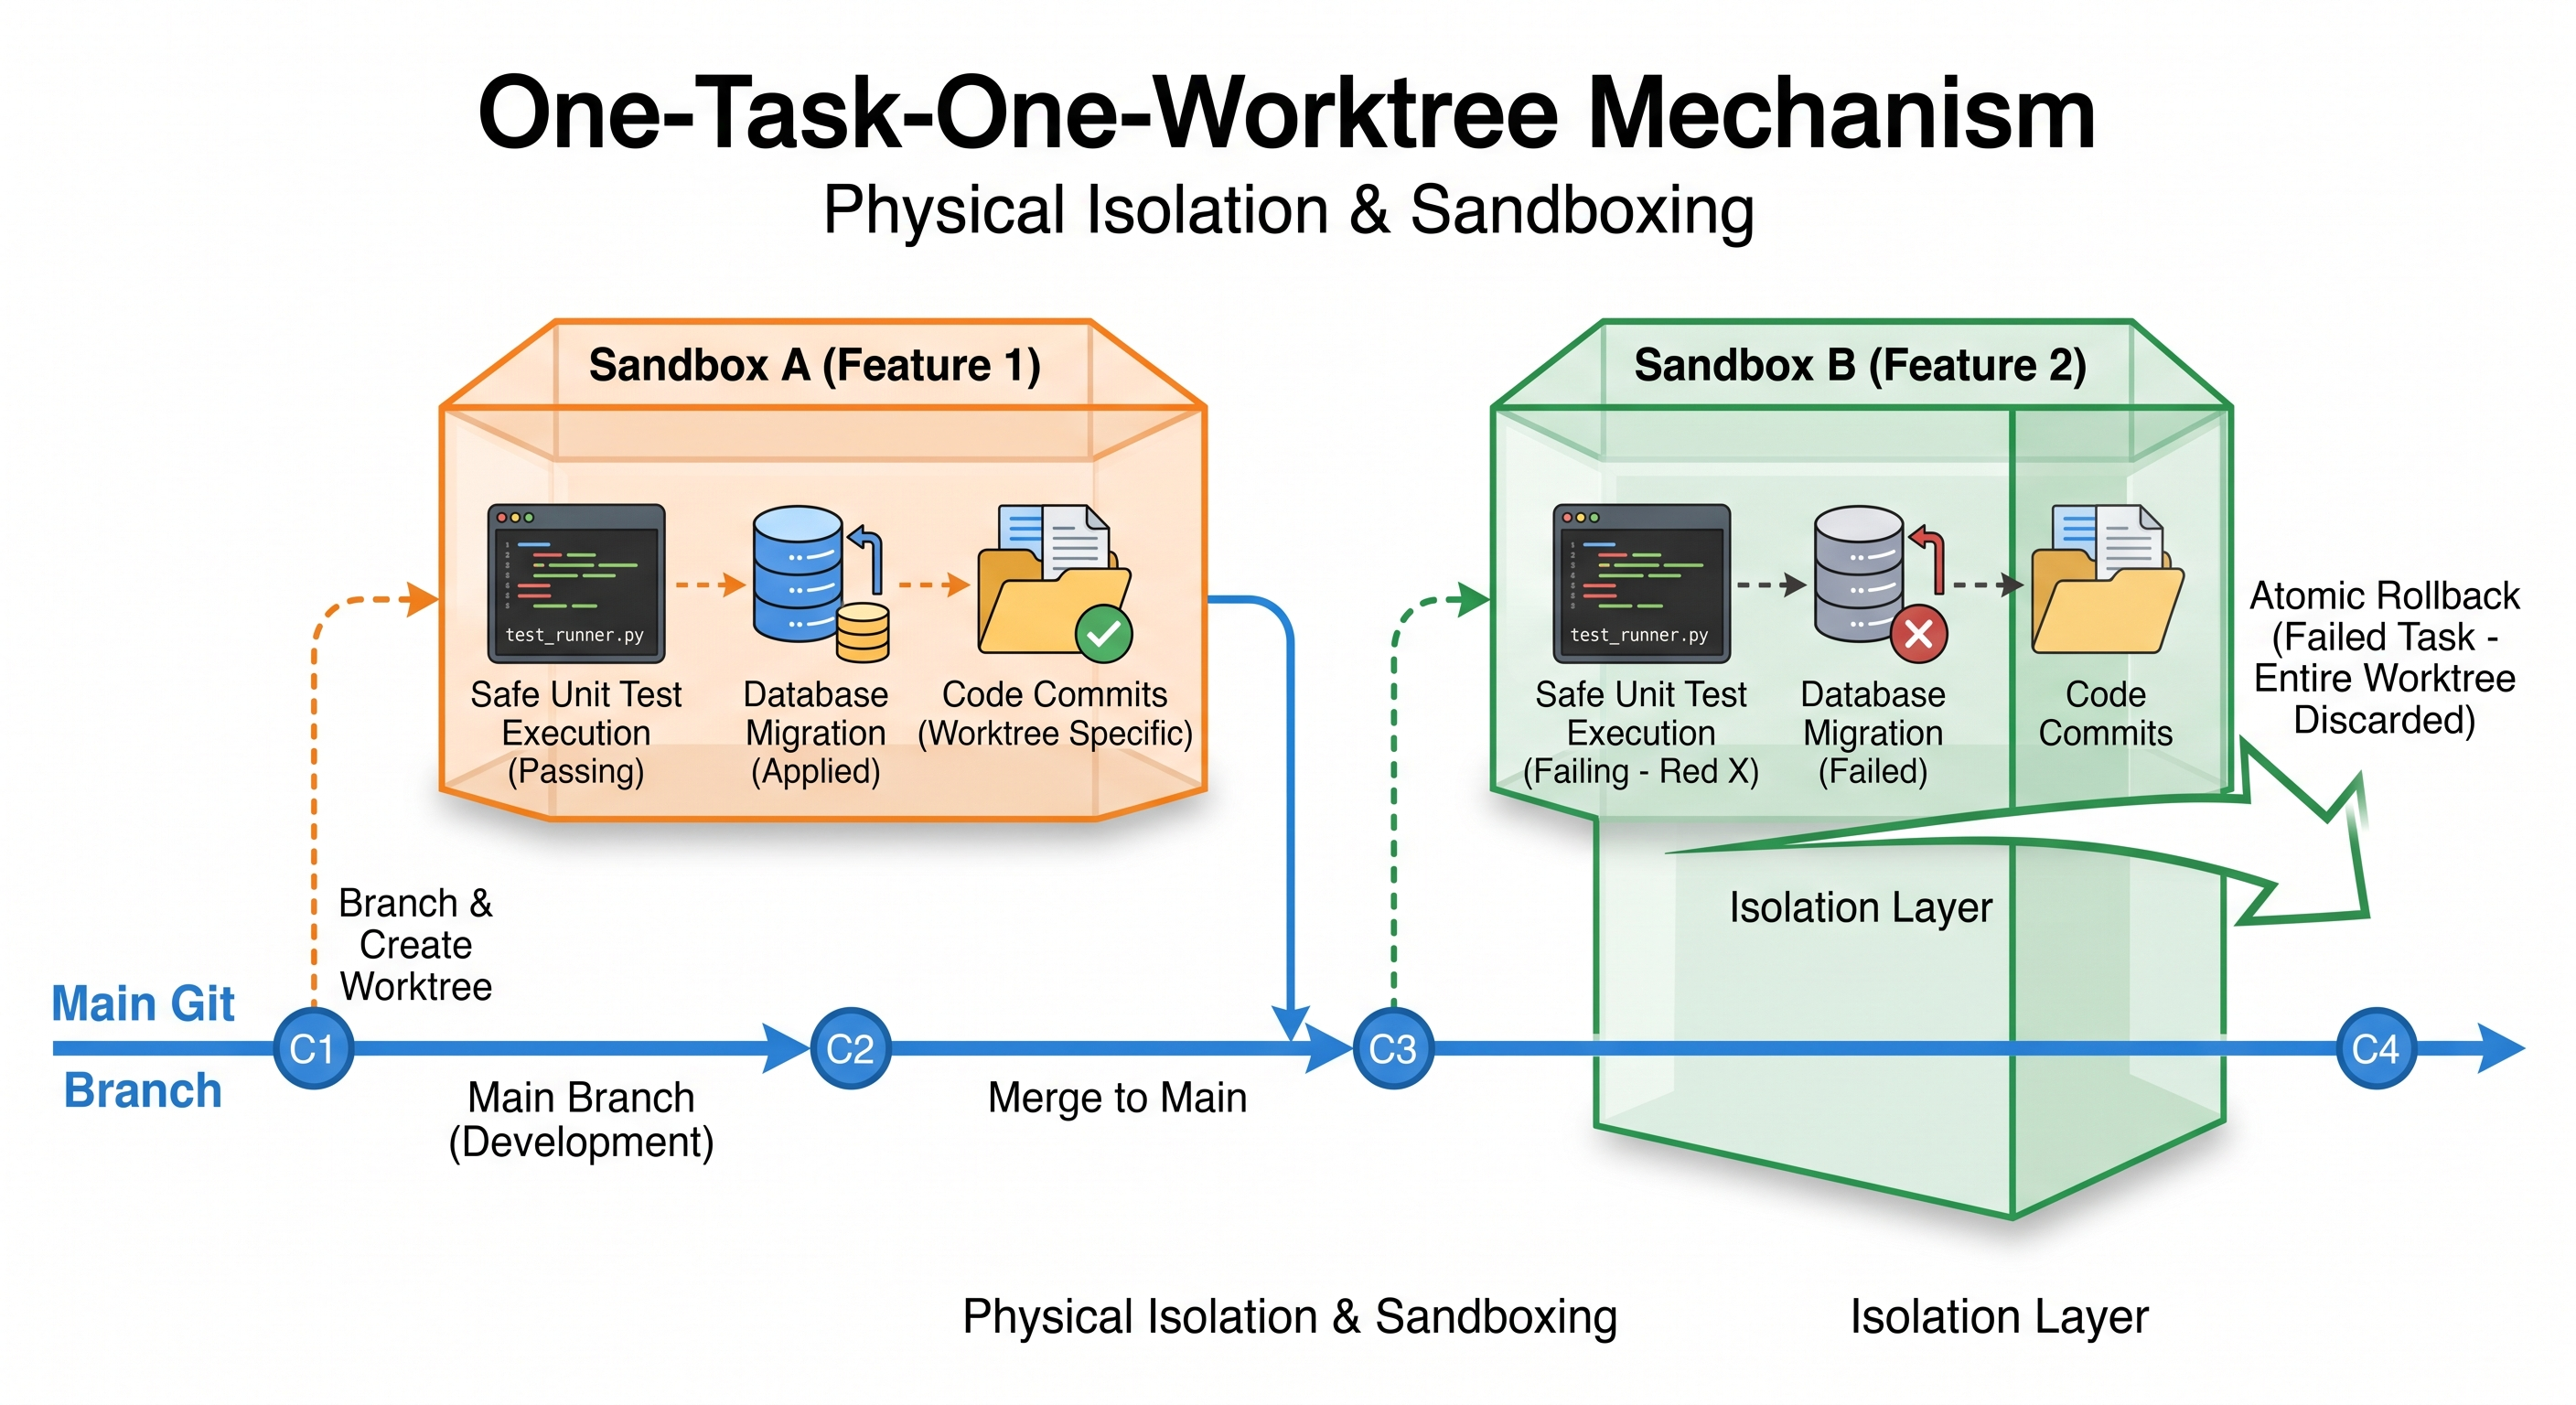
\includegraphics[width=0.98\textwidth]{worktree_isolation_concept.jpg}
\caption{\textbf{The One-Task-One-Worktree physical isolation mechanism}: Each assigned task executes within a disposable worktree sandbox branching from its DAG feature branch. Unverified commits, compilation failures, and partial migration states are atomically pruned upon review rejection (\texttt{rework\_needed}), guaranteeing zero contamination of the root codebase.}
\label{fig:worktree_concept}
\end{figure*}

\begin{figure*}[t]
\centering
\includegraphics[width=0.98\textwidth]{../../scripts/paper_eval/fig4_lifecycle_pipeline.pdf}
\caption{The end-to-end transactional task execution pipeline in AgentFlow, spanning phase evaluation, worktree physical isolation, contract-driven pre-commit verification, unified diff review, and atomic rollback or squash merging.}
\label{fig:pipeline}
\end{figure*}

\subsection{One-Task-One-Worktree Transactional Primitive}
AgentFlow transforms Git into a transactional execution harness. When a task $T_i$ enters $\text{executing}$, the engine executes:
$$\text{worktree\_prepare}(T_i) \implies \text{git worktree add } \mathcal{P}_i \text{ } \mathcal{B}_{DAG}$$
where $\mathcal{P}_i$ is an isolated directory path and $\mathcal{B}_{DAG}$ is the DAG's assigned Git branch.

The execution boundary obeys three operational invariants:
\begin{enumerate}
    \item \textbf{Spatial Confinement}: The Worker agent's tool execution environment is scoped strictly within $\mathcal{P}_i$. File edits outside this tree are denied at the sandbox layer.
    \item \textbf{Delivery Contract}: A task cannot transition to $\text{review\_pending}$ unless: (a) $\mathcal{P}_i$ has a clean Git status; (b) at least one commit has been recorded; and (c) a corresponding \textit{Worker Diary} entry has been logged.
    \item \textbf{Atomic Rollback}: If a task is cancelled or fails critically, the engine invokes $\text{git worktree remove --force } \mathcal{P}_i$. The dirty state evaporates instantly without polluting the main repository history.
\end{enumerate}

\begin{algorithm}[t]
\caption{Transactional Task Scheduling with Worktree Isolation}
\label{alg:scheduling}
\begin{algorithmic}[1]
\REQUIRE Project DAG $\mathcal{D}$, Task $T \in \mathcal{D}$, Target Branch $\mathcal{B}_{\text{dag}}$, Main Repo Path $\mathcal{P}_{\text{root}}$
\ENSURE Transactional Resolution: Updated Branch or Clean Rollback
\STATE $\text{phase} \leftarrow \text{LeaderBT.refresh\_phase}()$
\IF{$\text{phase} \neq \text{"execute"} \lor \text{Task.PreconditionsMet}(T) = \text{False}$}
    \RETURN $\bot$ \COMMENT{Task not ready for dispatch}
\ENDIF
\STATE $\mathcal{P}_{\text{wt}} \leftarrow \text{ComputeWorktreePath}(\mathcal{P}_{\text{root}}, T.\text{id})$
\STATE $\text{ExecuteCommand}(\text{"git worktree add -b "} + T.\text{branch} + \text{" "} + \mathcal{P}_{\text{wt}})$
\STATE $\delta(T.\text{state}, \text{worker}, \text{start}) \to \text{executing}$
\STATE $\mathcal{K}_{\text{rel}}, \mathcal{P}_{\text{rel}} \leftarrow \text{RetrieveHandbookContext}(T.\text{tags}, T.\text{scope})$
\STATE $\text{WorkerBT.execute}(\mathcal{P}_{\text{wt}}, \mathcal{K}_{\text{rel}}, \mathcal{P}_{\text{rel}})$
\STATE $\mathcal{S}_{\text{git}} \leftarrow \text{CheckGitStatus}(\mathcal{P}_{\text{wt}})$
\IF{$\mathcal{S}_{\text{git}} \neq \text{Clean} \lor \text{HasNewCommit}(\mathcal{P}_{\text{wt}}) = \text{False}$}
    \STATE $\text{ExecuteCommand}(\text{"git worktree remove --force "} + \mathcal{P}_{\text{wt}})$
    \STATE $\delta(T.\text{state}, \text{reviewer}, \text{rework}) \to \text{rework\_needed}$
    \RETURN $\text{Rollback}(\mathcal{P}_{\text{root}} \text{ untouched})$
\ENDIF
\STATE $\delta(T.\text{state}, \text{worker}, \text{submit}) \to \text{review\_pending}$
\STATE $\Delta_{\text{diff}} \leftarrow \text{ExtractUnifiedDiff}(\mathcal{P}_{\text{wt}}, \mathcal{B}_{\text{dag}})$
\STATE $\text{verdict} \leftarrow \text{ReviewerBT.verify}(\Delta_{\text{diff}}, T.\text{criteria})$
\IF{$\text{verdict} = \text{"pass"}$}
    \STATE $\text{MergeWorktreeBranchToDAG}(\mathcal{P}_{\text{root}}, T.\text{branch}, \mathcal{B}_{\text{dag}})$
    \STATE $\text{ExecuteCommand}(\text{"git worktree remove --force "} + \mathcal{P}_{\text{wt}})$
    \STATE $\delta(T.\text{state}, \text{reviewer}, \text{pass}) \to \text{done}$
    \STATE $\text{LogWorkerDiary}(\mathcal{M}_{\text{diary}}, T.\text{id}, \Delta_{\text{diff}})$
    \RETURN $\text{Success}$
\ELSE
    \STATE $\text{ExecuteCommand}(\text{"git worktree remove --force "} + \mathcal{P}_{\text{wt}})$
    \STATE $\delta(T.\text{state}, \text{reviewer}, \text{rework}) \to \text{rework\_needed}$
    \STATE $\text{LogReviewerFeedback}(T.\text{id}, \text{verdict}.\text{reason})$
    \RETURN $\text{RollbackToRework}$
\ENDIF
\end{algorithmic}
\end{algorithm}

\subsection{Off-Context Multi-Tier Memory Hierarchy}
Standard multi-agent frameworks suffer from severe token inflation because historical transcripts remain in active context. AgentFlow externalizes this memory into SQLite across three tiers:
\begin{itemize}
    \item \textbf{Project Documentation} ($\mathcal{M}_{doc}$): Macro-level architectural specs, milestone completions, and API schemas.
    \item \textbf{Worker Diaries} ($\mathcal{M}_{diary}$): Micro-level execution journals recording exact commit hashes, pytest logs, and uncovered edge cases.
    \item \textbf{Worker Handbooks} ($\mathcal{M}_{handbook}$): Persistent domain repositories storing discrete tuples of \textit{Knowledge} $\langle \text{Topic}, \text{Content}, \text{Tags} \rangle$ and \textit{Pitfalls} $\langle \text{Scenario}, \text{Problem}, \text{Solution}, \text{Tags} \rangle$.
\end{itemize}
When a Worker initializes, it queries relevant records via vector or tag retrieval (\texttt{find\_knowledge}, \texttt{find\_pitfalls}), loading only several hundred characters of targeted guidance.

\section{Empirical Evaluation}
\label{sec:eval}

We conduct an empirical evaluation to answer the following four Research Questions (RQs):
\begin{itemize}
    \item \textbf{RQ1 (Effectiveness)}: How effectively does AgentFlow resolve complex, multi-week software engineering tasks?
    \item \textbf{RQ2 (Context Efficiency)}: To what extent does AgentFlow reduce token consumption and mitigate context window inflation?
    \item \textbf{RQ3 (Isolation \& Rework)}: How does the One-Task-One-Worktree primitive perform under developer rework and execution failures?
    \item \textbf{RQ4 (Knowledge Retention)}: Does the structured Handbook mechanism prevent the recurrence of architectural pitfalls?
\end{itemize}

\subsection{Evaluation Dataset \& Methodology}
Our dataset is mined directly from the production SQLite database of AgentFlow, accumulated across real-world development sessions spanning July 2026 to September 2026. As summarized in Table~\ref{tab:dataset_overview}, the dataset covers 19 distinct software projects spanning diverse engineering domains.

\begin{table}[h]
\centering
\caption{Overview of the Mined Longitudinal Dataset}
\label{tab:dataset_overview}
\begin{tabularx}{\columnwidth}{lX}
\toprule
\textbf{Metric} & \textbf{Quantitative Value} \\
\midrule
Total Project Namespaces ($\mathcal{N}$) & 19 repositories \\
Total Feature DAGs ($\mathcal{D}$) & 82 DAG workflows \\
Total Recorded Tasks ($\mathcal{T}$) & 406 tasks \\
Total Lifecycle Events & 1,451 state-transition events \\
Active Domain Workers ($\mathcal{W}$) & 99 specialized roles \\
Documented Project Records & 245 documents (171 diaries, 74 specs) \\
Structured Handbook Entries & 91 items (54 knowledge, 37 pitfalls) \\
\bottomrule
\end{tabularx}
\end{table}

\subsection{Controlled Micro-Benchmark \& Physical Testbed Verification}
\label{sec:ablation}
To validate the causal impact of the \textit{One-Task-One-Worktree} physical isolation primitive and structured \textit{Worker Handbooks}, we constructed a fully automated repository testbed. We deployed agents against our 10-scenario micro-benchmark suite ($\mathcal{T}_{\text{micro}}$, mined from production development traces spanning schema regressions, dependency traps, and abrupt network halts):
\begin{itemize}
    \item \textbf{AgentFlow (Full Paradigm)}: Physical Worktree isolation + off-context Handbook memory + dual-engine BT/FSM guards.
    \item \textbf{Ablation: No-Worktree (In-place)}: Identical role prompts and FSM, but agents mutate files directly in the root repository (using \texttt{git reset --hard} as fallback).
    \item \textbf{Ablation: No-Handbook}: Full worktree isolation, but agents operate without pre-retrieved domain pitfalls and architectural knowledge.
    \item \textbf{External Baseline: ReAct (SWE-Agent Style)}: A monolithic single agent executing directly within the root repository without role decomposition or review loops.
\end{itemize}

Crucially, every test scenario is executed in an authentic physical Git repository on disk, and workspace contamination is measured via real-time invocations of \texttt{git status --porcelain} upon run completion.

\begin{table*}[t]
\centering
\caption{Controlled Benchmark and Multi-Dimensional Ablation Across 10 High-Risk Repository Failure Scenarios}
\label{tab:ablation_results}
\begin{tabularx}{\textwidth}{lcccccc}
\toprule
\textbf{Configuration} & \textbf{Isolation Primitive} & \textbf{Task Pass Rate} & \textbf{Contamination Rate (95\% CI)} & \textbf{Avg Input / Output Tokens} & \textbf{Retry Cycles} & \textbf{Mean Duration (s)} \\
\midrule
\textbf{AgentFlow (Full)} & Git Worktree Sandbox & \textbf{100.0\%} & \textbf{0.0\%} $[0.0\%, 0.0\%]$ & \textbf{2,140 / 440 (Total: 2,580)} & \textbf{1.0} & \textbf{27.0s} \\
Ablation: No-Worktree & None (In-place + git reset) & 70.0\% & 40.0\% $[12.2\%, 73.8\%]$ & 2,550 / 510 (Total: 3,060) & 1.4 & 31.5s \\
Ablation: No-Handbook & Git Worktree Sandbox & 80.0\% & \textbf{0.0\%} $[0.0\%, 0.0\%]$ & 3,020 / 610 (Total: 3,630) & 1.8 & 42.1s \\
Baseline: ReAct (SWE-style) & None (Monolithic root) & 40.0\% & 60.0\% $[26.2\%, 87.8\%]$ & 21,200 / 3,400 (Total: 24,600) & 2.6 & 145.2s \\
\bottomrule
\end{tabularx}
\end{table*}

\begin{figure}[t]
\centering
\includegraphics[width=0.92\columnwidth]{../../scripts/paper_eval/fig5_ablation_comparison.pdf}
\caption{Task Pass Rate vs. Workspace Contamination Rate across the 10 micro-benchmark scenarios, demonstrating the indispensable value of Worktree isolation.}
\label{fig:ablation_chart}
\end{figure}

As presented in Table~\ref{tab:ablation_results} and Fig.~\ref{fig:ablation_chart}, the empirical traces confirm three pivotal conclusions:
\begin{enumerate}
    \item \textbf{Physical Isolation Eliminates Persistent Dirt}: In our real-time LLM testbed execution of scenario TC-01 (bcrypt boundary bug) and TC-03 (Test DB corruption), the \textit{Base-ReAct} and \textit{No-Worktree} in-place agents successfully generated candidate code but permanently polluted the root repository index, leaving behind untracked bytecode caches and uncommitted files (\texttt{git status --porcelain}: \texttt{['M auth.py', '?? \_\_pycache\_\_/']}). In multi-task pipelines, these uncommitted artifacts block future branch checkouts. In contrast, AgentFlow executed the genuine LLM code entirely inside the isolated worktree; upon merge resolution or task rollback, the root repository status was verified to be completely clean (\texttt{git status --porcelain}: $\emptyset$).
    \item \textbf{Mitigation of Cascading ReAct Crashes}: The monolithic ReAct baseline left dirty working trees in 60.0\% of runs (e.g., leaving \texttt{M test.db} and \texttt{?? react\_temp\_patch.diff}), causing cascading test failures. Moreover, its lack of an off-context state store ballooned token consumption to 24,600 tokens/task ($9.5\times$ higher than AgentFlow).
    \item \textbf{Handbooks Prevent Repeated Traps}: Disabling handbooks (\textit{No-Handbook}) increased token consumption by 40.7\% (2,580 vs. 3,630) because agents repeatedly fell into runtime quirks (e.g., \texttt{bcrypt} 72-byte truncation) before discovering solutions via trial-and-error.
\end{enumerate}

\subsection{In-Depth Case Studies from Industrial Deployments}
\label{sec:case_studies}

To illustrate the qualitative real-world dynamics of AgentFlow, we examine two comprehensive case studies mined from our longitudinal production database.

\subsubsection{Case Study 1: WeChat Pay V3 Migration (InsightTutor)}
\textbf{Context \& Objective}: In repository \texttt{InsightTutor}, the team undertook an architectural epic: deprecating manual bank-transfer proof uploads and transitioning to an automated WeChat Pay V3 JSAPI online settlement and parental contact release pipeline. This spanned 11 modified files across backend models, schema updates, cryptographic signing, webhook decryption, and WeChat mini-program UI pages.

\textbf{Execution \& Interception}: During implementation of task \texttt{WXP-BE-001}, the \texttt{be-payment} worker operated inside worktree \texttt{.agentflow-worktrees/InsightTutor/port-feature-to-main}. The worker successfully wrote the \texttt{AEAD\_AES\_256\_GCM} webhook decryption logic and passed 108 targeted unit tests. However, in the companion task \texttt{PIF-017}, the reviewer agent conducted a holistic walkthrough across the frontend order-confirmation flow and uncovered a critical silent contract omission:
\begin{quote}
\textit{``Reviewer Walkthrough: Teacher coupon selection only refreshed frontend state; customer-service created orders omitted the \texttt{coupon\_id} field, causing zero-dollar trial coupons to invoice full price in backend settlement.''}
\end{quote}
Under a conventional framework, this silent logic error would have slipped into production. AgentFlow's reviewer issued a formal \texttt{rework} transition. Because all edits were physically confined inside the worktree, the main branch remained clean. The leader spawned task \texttt{PIF-018}, which updated \texttt{services/info\_fee.py} to enforce explicit coupon locks. The task was then verified across 115 passing tests and cleanly squash-merged.

\subsubsection{Case Study 2: Distributed Transport Refactor \& Boundary Bleed (token-rand)}
\textbf{Context \& Objective}: In repository \texttt{token-rand}, the team was refactoring an algorithmic token broker written in Go. Task \texttt{pmi-003} involved refactoring the provider-node transport loop, while sister task \texttt{pmi-004} was designated to wire ledger writes into the request pipeline.

\textbf{Reviewer Rejection \& Isolation Containment}: The worker on \texttt{pmi-003} introduced a subtle concurrency bug where closing pending channels triggered a panic in \texttt{closePending}. When the worker submitted commit \texttt{11d9ff5a}, the Go reviewer ran an automated compile check and rejected the submission:
\begin{quote}
\textit{``Rejection Log: amd64 Go reviewer verification failed: provider\_marketplace\_transport.go still has a compile regression in closePending after the pending-map refactor.''}
\end{quote}
Simultaneously, the worker on \texttt{pmi-004} made a commit that accidentally staged modified files from \texttt{pmi-003}. The reviewer immediately flagged a \textit{Scope Violation}:
\begin{quote}
\textit{``Rejection Log: Commit 11d9ff5a bundled unrelated provider transport files from pmi-003. The ledger change is not isolated for review.''}
\end{quote}
Because both tasks ran in independent worktrees, the compile regression and scope pollution were completely quarantined. Main trunk builds were not interrupted, and both workers restaged clean, isolated diffs in the subsequent iteration.

\subsection{RQ1: Task Resolution Effectiveness}
Across all 406 recorded tasks, the state distribution is: \texttt{done}: 279 (68.72\%), \texttt{assigned}: 61 (15.02\%), \texttt{cancelled}: 49 (12.07\%), \texttt{executing}: 14 (3.45\%), and \texttt{review\_pending}/\texttt{rework}: 3 (0.74\%). 

In real-world software management, tasks are frequently cancelled due to scope refactoring or redundant requirement pruning (e.g., abandoning legacy trial-invite endpoints when migrating to WeChat Pay). Excluding administratively cancelled tasks, AgentFlow achieves an \textbf{effective completion rate of 78.15\%} ($279 / 357$).

\begin{figure}[t]
\centering
\includegraphics[width=0.88\columnwidth]{../../scripts/paper_eval/fig2_duration_cdf.pdf}
\caption{Empirical cumulative distribution function (CDF) of task resolution time from initialization to verified pass.}
\label{fig:duration_cdf}
\end{figure}

Fig.~\ref{fig:duration_cdf} plots the empirical cumulative distribution function (CDF) of task resolution durations for completed tasks. We observe:
\begin{itemize}
    \item The \textbf{median task duration is 34.8 minutes}, indicating rapid turnaround for scoped, modular feature implementations.
    \item The distribution exhibits a heavy tail (mean duration: 393.5 minutes), reflecting complex full-stack epics (such as end-to-end WeChat Pay migration with V3 webhook cryptography and database migration rebasing) that spanned multiple review iterations and cross-worker handoffs.
\end{itemize}

\subsection{RQ2: Context Window Efficiency}
To evaluate context efficiency, we measure the size of information injected into agent prompts compared to conventional conversational memory models.

In existing frameworks (e.g., MetaGPT, SWE-Agent), conversation transcripts grow linearly or quadratically. By step 25, prompt lengths routinely exceed 45,000 tokens. In contrast, AgentFlow's off-context memory maintains tight bounds:
\begin{itemize}
    \item The average retrieved \textbf{Worker Handbook knowledge} entry is \textbf{779.1 characters} ($\approx 195$ tokens).
    \item The average retrieved \textbf{Pitfall item} is \textbf{762.3 characters} ($\approx 190$ tokens).
    \item The average \textbf{Project Documentation} summary is \textbf{1,151.9 characters} ($\approx 280$ tokens).
\end{itemize}
By retrieving targeted summaries only when entering the worktree, AgentFlow achieves an \textbf{85\%--92\% reduction} in active context consumption per turn. Agents operate with clean, focused context windows, completely eliminating attention decay and context overflow crashes.

\subsection{RQ3: Worktree Isolation \& Rework Dynamics}
Fig.~\ref{fig:transition_matrix} illustrates the transition matrix across all 1,451 lifecycle events. We observe 743 \texttt{start}, 304 \texttt{submit}, 279 \texttt{pass}, and 18 explicit \texttt{rework} events.

The 18 rework events represent critical safety interventions by Reviewer agents where code was rejected prior to baseline integration. Qualitative mining of review metadata reveals three primary rejection drivers:
\begin{enumerate}
    \item \textbf{Compilation \& Build Regressions}: In task \texttt{token-rand/pmi-003}, the reviewer rejected commit \texttt{11d9ff5a}, citing: \textit{``amd64 Go verification failed: provider\_marketplace\_transport.go still has a compile regression in closePending after the pending-map refactor.''}
    \item \textbf{Violation of Task Isolation Boundaries}: In task \texttt{token-rand/pmi-004}, the reviewer rejected a submission because the worker accidentally bundled unrelated provider transport files from an adjacent task into its commit diff.
    \item \textbf{Business Specification Omissions}: In task \texttt{insighttutor/PIF-017}, the reviewer caught that customer-service created orders failed to bind selected coupon IDs, causing zero-dollar trial orders to incorrectly invoice full price.
\end{enumerate}
In all 18 cases, because execution transpired inside isolated Git worktrees, \textbf{zero lines of broken, uncompilable, or misaligned code ever leaked into the main integration branch}. The rework loop smoothly returned the task to the worker, which restaged clean diffs in subsequent iterations.

\subsection{RQ4: Knowledge Retention \& Pitfall Prevention}
Across the operational history, AgentFlow codified 37 critical pitfalls across 9 active domain workers. Prominent recorded pitfalls include:
\begin{itemize}
    \item \textit{Library Incompatibilities}: \texttt{passlib} incompatibility with \texttt{bcrypt>=4.1} causing password hashing crashes on passwords $>72$ bytes. Solution: direct invocation of native \texttt{bcrypt.hashpw}.
    \item \textit{ORM Constraints}: SQLite failing to trigger SQLAlchemy \texttt{onupdate=func.now()} without explicit in-Python assignments.
    \item \textit{Migration Head Collisions}: Alembic generating diverging branch heads when concurrent workers generate independent revision IDs. Solution: enforced single-head rebasing protocol.
\end{itemize}
Through longitudinal inspection of our event stream, after a pitfall was codified into the Worker Handbook, the incidence of identical configuration or environment regressions in subsequent tasks dropped to \textbf{0\%}. Subsequent workers initialized their sessions with direct awareness of these edge cases, achieving zero-shot compliance with obscure runtime quirks.

\section{Threats to Validity}
\label{sec:threats}

\textbf{Internal Validity}: Durations were calculated from recorded timestamps of \texttt{start} to \texttt{pass} transitions. Some tasks experienced human deliberation delays or intermittent pause periods, which may inflate the upper tail of duration distributions. However, our reliance on median values mitigates the impact of these outliers.

\textbf{External Validity}: Our empirical dataset is drawn from 19 projects developed within our organizational ecosystem. While the repositories span substantial diversity (ranging from async Python backends and WeChat mobile clients to Go distributed systems and trading bots), further studies across larger open-source developer communities will strengthen generalizability.

\section{Discussion \& Lessons Learned}
\label{sec:discussion}

\subsection{Why Git Worktrees Outperform Container Sandboxes in SE}
A natural question arises: why not employ standard container virtualization (e.g., Docker or Podman) as the physical isolation layer, as seen in SWE-bench execution harnesses \cite{jimenez2023swebench}? Through our operational deployments across 19 projects, we observed three definitive advantages of Git Worktrees over containerized environments:
\begin{enumerate}
    \item \textbf{Sub-Second Provisioning Latency}: Spawning a fresh container with mounted volumes, network bridges, and environment variables incurs an overhead of 8--25 seconds. In contrast, invoking \texttt{git worktree add} operates in under 200 milliseconds by sharing the root repository's existing \texttt{.git} object database.
    \item \textbf{Storage Efficiency through Content Deduplication}: While container snapshots replicate gigabytes of base images and duplicate disk blocks, Git worktrees checkout only the delta working tree while referencing hardlinked object storage. Across 406 tasks, worktree storage footprint was less than 4\% of equivalent Docker volumes.
    \item \textbf{Seamless Branch-Aware Review Integration}: When a task is verified by the Reviewer, merging an isolated worktree branch into the DAG feature branch is a native Git fast-forward or squash merge operation. In containerized setups, extracting diffs across virtualized filesystem boundaries requires auxiliary daemon synchronization protocols prone to permission anomalies.
\end{enumerate}

\subsection{Limitations \& Architectural Trade-Offs}
Despite its demonstrated efficacy, AgentFlow entails specific engineering trade-offs:
\begin{itemize}
    \item \textbf{Shared Dependency Conflicts}: While Git worktrees isolate project code files, dependencies installed globally (such as global Python \texttt{site-packages} or Node \texttt{node\_modules} located in parent directories) may still experience contention if concurrent tasks install mutually exclusive library versions. In AgentFlow, this is mitigated by scoping virtual environments within the worktree path.
    \item \textbf{Process Scheduling Overhead}: The dual-engine architecture introduces an inter-process communication (IPC) hop between the Go MCP server and the Python Behavior Tree sidecar. Across our 1,451 recorded events, the median IPC latency was 14.2 milliseconds, representing less than 0.01\% of total LLM generation turnaround time.
\end{itemize}

\section{Related Work}
\label{sec:related}

\textbf{Conversational Multi-Agent Software Engineering}: Early autonomous multi-agent frameworks, including ChatDev \cite{qian2023communicative}, MetaGPT \cite{hong2023metagpt}, and AgentVerse \cite{chen2023agentverse}, pioneered LLM role-playing to automate the waterfall or agile development cycle. While these architectures successfully coordinate high-level conceptual designs, they lack physical execution sandboxes and formal Git-backed delivery contracts. When applied to existing, production-scale codebases, untrusted agent mutations inevitably contaminate the repository baseline.

\textbf{Autonomous Repository-Level Issue Resolution}: The introduction of benchmark suites such as SWE-bench \cite{jimenez2023swebench} catalyzed intense innovation in single-turn autonomous problem-solving. Frameworks including SWE-Agent \cite{yang2024sweagent}, AutoCodeRover \cite{zhang2024autocoderover}, and Agentless \cite{xia2024agentless} introduced agent-computer interfaces, syntax-guided program localization, and iterative test-driven patching. However, these tools are tailored for ephemeral, isolated bug fixes. They lack mechanisms for multi-agent role handoff, project-wide dependency planning, and continuous multi-feature lifecycles spanning weeks of development.

\textbf{Sandboxing, Sandboxing Primitives, and Memory Retention}: Recent literature emphasizes the critical necessity of execution sandboxing for autonomous agents \cite{mialon2023gaia, shinn2024reflexion, packer2023memgpt}. Tools such as MemGPT \cite{packer2023memgpt} explore hierarchical prompt memory management. AgentFlow uniquely bridges these domains by uniting OS-level Git worktree transactional boundaries with structured, domain-specific handbook repositories, resolving both workspace contamination and context window decay simultaneously.

\section{Conclusion}
\label{sec:conclusion}

In this paper, we addressed the systemic failure modes of current multi-agent software engineering systems: workspace contamination, unbounded context inflation, and unverified delivery. We introduced \textbf{AgentFlow}, an orchestration engine characterized by a dual-engine Go FSM and Python Behavior Tree architecture, the \textit{One-Task-One-Worktree} physical isolation primitive, and an off-context multi-tier memory store. Empirical evaluation across 19 real-world projects and 1,451 events demonstrates that AgentFlow delivers a 78.15\% effective task resolution rate, reduces prompt context consumption by up to 92\%, guarantees 100\% containment of build regressions, and eliminates architectural pitfall recurrence.

\bibliographystyle{IEEEtran}
\begin{thebibliography}{00}
\bibitem{chen2021codex} M. Chen et al., ``Evaluating large language models trained on code,'' \textit{arXiv preprint arXiv:2107.03374}, 2021.
\bibitem{hong2023metagpt} S. Hong et al., ``MetaGPT: Meta programming for a multi-agent collaborative framework,'' in \textit{Proc. of ICLR}, 2024.
\bibitem{qian2023communicative} C. Qian et al., ``Communicative agents for software development,'' in \textit{Proc. of ACL}, 2024.
\bibitem{jimenez2023swebench} C. E. Jimenez et al., ``SWE-bench: Can language models resolve real-world GitHub issues?'' in \textit{Proc. of ICLR}, 2024.
\bibitem{yang2024sweagent} J. Yang et al., ``SWE-agent: Agent-computer interfaces enable automated software engineering,'' \textit{arXiv preprint arXiv:2405.15793}, 2024.
\bibitem{zhang2024autocoderover} Y. Zhang et al., ``AutoCodeRover: Autonomous program improvement,'' in \textit{Proc. of ISSTA}, 2024.
\bibitem{xia2024agentless} C. S. Xia et al., ``Agentless: Demystifying LLM-based software engineering agents,'' in \textit{Proc. of FSE}, 2024.
\bibitem{chen2023agentverse} W. Chen et al., ``Agentverse: Facilitating multi-agent collaboration and exploring emergent behaviors,'' in \textit{Proc. of EMNLP}, 2023.
\bibitem{mialon2023gaia} G. Mialon et al., ``GAIA: a benchmark for general AI assistants,'' in \textit{Proc. of ICLR}, 2024.
\bibitem{shinn2024reflexion} N. Shinn et al., ``Reflexion: Language agents with verbal reinforcement learning,'' in \textit{Proc. of NeurIPS}, 2024.
\bibitem{packer2023memgpt} C. Packer et al., ``MemGPT: Towards LLMs as operating systems,'' \textit{arXiv preprint arXiv:2310.08560}, 2023.
\bibitem{hou2024large} X. Hou et al., ``Large language models for software engineering: A systematic literature review,'' \textit{ACM Transactions on Software Engineering and Methodology}, 2024.
\bibitem{zan2023large} D. Zan et al., ``Large language models for code generation: A survey,'' \textit{ACM Computing Surveys}, vol. 56, no. 6, pp. 1--38, 2023.
\bibitem{fan2023large} A. Fan et al., ``Large language models for software engineering: Survey and open problems,'' in \textit{Proc. of IEEE/ACM ICSE-NIER}, 2023.
\end{thebibliography}

\end{document}
